\documentclass[aspectratio=43,11pt]{beamer}
\usepackage[T1]{fontenc}
\usepackage[utf8]{inputenc}
\usepackage{lmodern}
\usepackage{xcolor}
% \usepackage[margin=1in]{geometry}
\usepackage{graphicx}
\usepackage{caption}
\usepackage{subcaption}
\usepackage{float}
\usepackage[french]{babel}
\usepackage{listings}
\usepackage{tabularx}
\usepackage{hyperref}
\usepackage{mathtools}
\usepackage{fancyhdr}
\usepackage{lastpage}
\usepackage{amsfonts}
\usepackage{verbatim} 
\setbeamercovered{transparent} 
\setbeamertemplate{frametitle continuation}{}
% \pagenumbering{alph}
% \usepackage{beamerthemesplit}
\beamertemplatenavigationsymbolsempty
% \usepackage{beamerthemeshadow}
\usetheme{Boadilla}
\usecolortheme{beaver}


\AtBeginSection[]{
  \begin{frame}
  \vfill
  \centering
  \begin{beamercolorbox}[sep=8pt,center,shadow=true,rounded=true]{title}
    \usebeamerfont{title}\insertsectionhead\par%
  \end{beamercolorbox}
  \vfill
  \end{frame}
}


% \setbeamercolor{block title}{bg=red!30,fg=black}
% \pagestyle{fancy}
% \fancyhf{}
 
% \rfoot{Page \thepage \hspace{1pt} of \pageref{LastPage}}
% \pagenumbering{⟨style⟩}
\hypersetup{
  colorlinks=true,
  linkcolor=black,
  filecolor=magenta,
  urlcolor=blue,
}
\graphicspath{ {./images/} }
\definecolor{codegreen}{rgb}{0,0.6,0}
\definecolor{codegray}{rgb}{0.5,0.5,0.5}
\definecolor{codepurple}{rgb}{0.58,0,0.82}
\definecolor{backcolour}{rgb}{0.95,0.95,0.92}
\definecolor{codeblue}{rgb}{0.1,0.4,0.6}

\lstdefinestyle{mystyle}{
    backgroundcolor=\color{backcolour},   
    commentstyle=\color{codegreen},
    keywordstyle=\color{magenta},
    numberstyle=\tiny\color{codegray},
    stringstyle=\color{codepurple},
    identifierstyle=\color{codeblue},
    basicstyle=\ttfamily\footnotesize,
    breakatwhitespace=false,         
    breaklines=true,                 
    captionpos=b,                    
    keepspaces=true,                 
    numbers=left,                    
    numbersep=5pt,                  
    showspaces=false, 
    showstringspaces=false,
    showtabs=false,                  
    tabsize=2
}
\lstset{style=mystyle}

\title{TIPE - La Ville}
\subtitle{Comment créer un réseau de transports publics dans une ville afin de minimiser les temps de déplacement ?}
\author{Valentin FOULON - N° 29836}
\date{\today}

\begin{document}
\begin{frame}
    \titlepage
\end{frame}
\begin{frame}{Table des matières}
    \tableofcontents
\end{frame}

\section{Choix du thème}

\section{Définitions}
\begin{frame}{Définitions}
    \begin{minipage}{0.7\textwidth}
    \begin{block}{Définition}
        Graphe : on note $G=(S, A)$ un graphe ayant pour sommets l'ensemble $S$ et pour arêtes l'ensemble $A$. On désigne par $|A|$ et $|S|$ les cardinaux respectifs de $A$ et $S$.
    \end{block}
    \end{minipage}
    \begin{minipage}{0.25\textwidth}
        \centering
    \includegraphics[width=0.7\textwidth]{graphe_complet}
    \end{minipage}
    \begin{exampleblock}{Remarque}
        On considère ici des graphes non orientés connexes : il n'y a pas de point isolé dans le graphe.
    \end{exampleblock}
\end{frame}
\begin{frame}{Définitions}
    \begin{block}{Définition}
        Poids d'une arête : fonction $d : A \rightarrow \mathbb{N}, (u, v) \rightarrowtail d(u, v)$ utilisée pour les algorithmes de graphe. On utilisera ici la distance euclidienne entre deux sommets.
    \end{block}
    On représente les villes par des graphes non orientés connexes. Les centres d'intérêt sont des sommets de ce graphe. Pour chaque couple (u, v) de sommets dans le graphe, si la distance entre u et v est inférieure à une valeur donnée, il existe une arête entre u et v. On suppose que le graphe ainsi créé reste connexe.
\end{frame}
\section{Objectifs du TIPE}
\begin{frame}{Objectifs}
    Etudier différents algorithmes pour créer un réseau de transport public et les comparer
    \begin{itemize}
        \item Les algorithmes doivent produire des résultats efficaces
        \item Les algorithmes doivent être efficaces
        \begin{itemize}
            \item On espère ici avoir une complexité inférieure à $O(n^2)$
        \end{itemize}
        \item Tous les points d'intérêt doivent être reliés entre eux
        \item La solution trouvée doit être réaliste
    \end{itemize}
\end{frame}
\section{Conditions d'exploitation}
\begin{frame}{Conditions d'exploitation}
    \begin{itemize}
        \item On utilise l'exemple des métros car pas de contrainte de parcours
        \item Les trains circulent à vitesse constante (proportionnalité entre distance et temps de trajet)
        \item Le temps d'arrêt à une station est nul
        \item Le temps d'attente à une station est nul
    \end{itemize}
    Ces suppositions ne sont pas réelles mais influent peu sur le résultat.
\end{frame}
\begin{frame}{Paramètres}
    Les unités sont arbitraires
    \begin{itemize}
        \item On utilise un plan de taille 100*100
        % \item On souhaite des distances inférieures à 15
        \item Pour les tests on positionne au plus 1000 stations de manière aléatoire
    \end{itemize}
\end{frame}
\section{Première approche : algorithme de Dijkstra}
\begin{frame}{Dijkstra}
    \begin{block}{Algorithme de Dijkstra}
        Algorithme de plus court chemin dans un graphe.
    \end{block}
    Objectif : trouver le plus court chemin entre les bords haut et bas du plan.
\end{frame}
\begin{frame}{Choix et utilisation de l'algorithme}
    \centering
    \includegraphics[width=0.4\textwidth]{maze1}
    \centering
    \includegraphics[width=0.4\textwidth]{maze2}
\end{frame}
\begin{frame}{Dijkstra}
    \begin{itemize}
        \item Complexité : $O(|A| log |A|)$
        \item Trouve le meilleur résultat à chaque fois
        \item Fonctionne car la fonction de poids est positive
    \end{itemize}
\end{frame}
\begin{frame}{Production de l'algorithme}
    \centering
        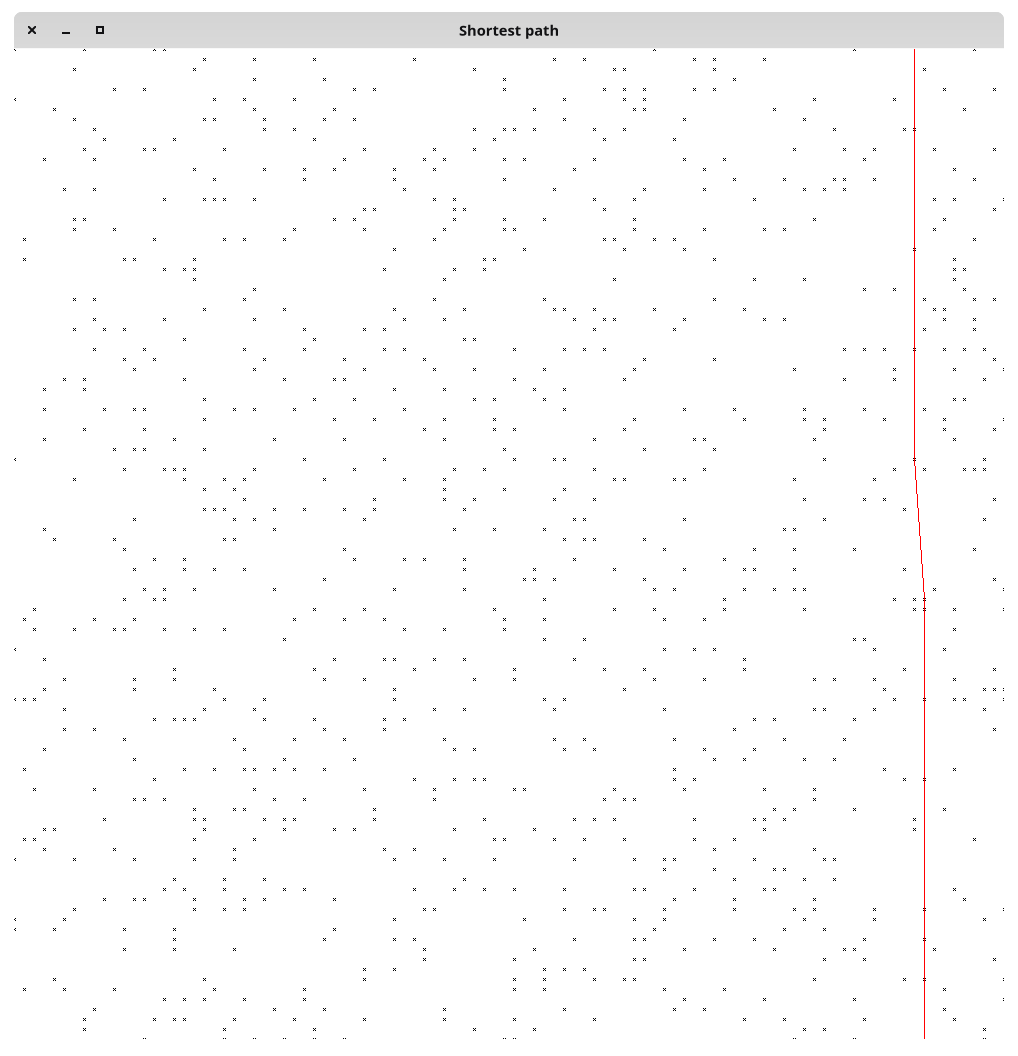
\includegraphics[width=0.5\textwidth]{sp}

    Cet algorithme crée des trajets avec peu de changements de direction.
\end{frame}
\begin{frame}{Mesure des résultats}
    Les différents algorithmes employés ici permettent de sauvegarder les graphes créés dans des fichiers.
    Un autre programme peut ensuite calculer les informations que l'on souhaite sur ces graphes : moyenne, médiane, longueur minimum, maximum.
\end{frame}
\begin{frame}{Résultat sur un jeu de données aléatoire}
    \centering
        \includegraphics[height=0.8\textheight]{sp_r}

\end{frame}
\begin{frame}{Problèmes}
    \begin{itemize}
        \item La solution trouvée est alors optimale en terme de temps de trajet
        \item La capacité de transport entre les deux points vaut $(|S| - 2) *$ "nombre de places dans une rame"
        \item Cet algorithme donne le plus court chemin entre deux points spécifiques du graphe, on peut ainsi l'appliquer sur chaque couple de sommets
        \item Mais il reste deux problèmes
        \begin{itemize}
            \item Risque de lignes en double sur des portions de trajet
            \item Beaucoup de lignes à créer
        \end{itemize}
    \end{itemize}
\end{frame}
\section{Deuxième approche : algorithme de Kruskal}
\begin{frame}{Kruskal}
    \begin{block}{Algorithme de Kruskal}
        Algorithme qui trouve un arbre couvrant de poids minimal dans un Graphe.
    \end{block}
    \begin{block}{Définition}
        Un arbre couvrant est un sous-graphe $G'=(S, A')$ de $G=(S, A)$ où $A' \subset A$ et pour tous $(u, v) \in A$, il existe un chemin de $u$ à $v$ dans $G'$.
    \end{block}
    \begin{exampleblock}{Remarque}
        Un arbre couvrant de poids minimum est \textbf{un} arbre couvrant dont la somme des poids des arêtes de $A'$ est la plus petite.
    \end{exampleblock}
\end{frame}
\begin{frame}{Choix et utilisation de l'algorithme}
\end{frame}
\begin{frame}{Kruskal}
    \begin{itemize}
        \item Complexité : $O(|A| log |A|)$
        \item Algorithme correct : le sous-graphe renvoyé est un arbre couvrant de poids minimum
    \end{itemize}
\end{frame}
\begin{frame}{Production de l'algorithme}
    \centering
        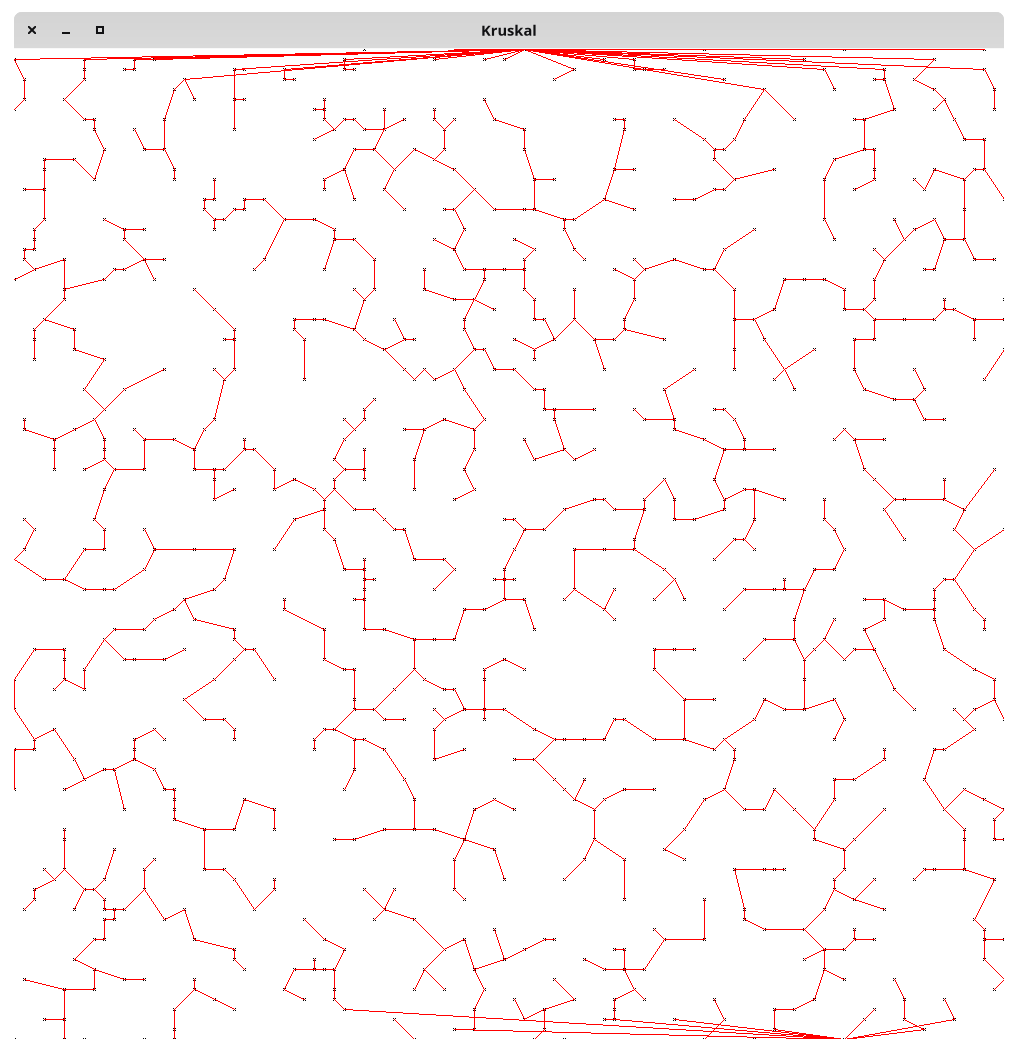
\includegraphics[width=0.5\textwidth]{k}

    Chaque sommet est relié à tous les autres par un chemin.
\end{frame}
\begin{frame}{Résultat sur un jeu de données aléatoire}
    \centering
        \includegraphics[height=0.8\textheight]{k_r}

    Une grande partie des chemins a une longueur faible.
\end{frame}
\begin{frame}{Problèmes}
    \begin{itemize}
        \item Cet algorithme fournit un unique chemin entre chaque couple de sommets sauf entre les sommets haut et bas
        \item La capacité de transport entre les deux points vaut le nombre de places dans une rame
        \item Certains chemins semblent donc absurdes et beaucoup trop longs entre certains couples de sommets
        \item On peut alors ajouter des arêtes avec l'algorithme de Dijkstra vu avant
        \item Beaucoup de lignes différentes à créer
    \end{itemize}
\end{frame}

\section{Troisième algorithme}

\begin{frame}{Résumé de ce qu'on a vu}
    Les deux algorithmes vu précédemment ne suffisent pas à répondre à la question.
    De plus les villes se développent en agglomérations, certaines lieux peuvent devenir des hubs.
\end{frame}

\begin{frame}{Idée}
    Utiliser l'algorithme des K-moyennes afin de regrouper des centres d'intérêt entre eux, relier les groupes entre eux puis relier les centres d'intérêt dans ces groupes.
\end{frame}
\begin{frame}{K-moyennes}
    \begin{block}{K-moyennes}
        Algorithme de regroupement de points en K groupes appelés clusters afin de minimiser la distance entre les points d'un même groupe.
    \end{block}
    \begin{exampleblock}{Remarque}
        On utilise ici de l'algorithme de Lloyd, ou algorithme naïf.
    \end{exampleblock}
\end{frame}
\begin{frame}{Choix et utilisation de l'algorithme}
\end{frame}
\begin{frame}{K-moyennes}
    \begin{itemize}
        \item Complexité : $O(|S| K i)$, i étant le nombre d'itérations avant d'obtenir une solution
        \item L'algorithme produit une solution souvent proche de l'optimale
    \end{itemize}
    \begin{alertblock}{Attention}
        L'algorithme ne converge pas nécessairement vers une solution pour certaines combinaisons de jeux de données, valeurs de K, positions initiales des centroïdes.
    \end{alertblock}
\end{frame}
\begin{frame}{Résultat sur un jeu de données aléatoire}
    \only<1>{
        \centering
            \includegraphics[width=0.5\textwidth]{m0}

        1e itération
    }
    \only<2>{
        \centering
            \includegraphics[width=0.5\textwidth]{m1}

        2e itération
    }
    \only<3>{
        \centering
            \includegraphics[width=0.5\textwidth]{m2}

        3e itération
    }
    \only<4>{
        \centering
            \includegraphics[width=0.5\textwidth]{m3}

        4e itération
    }
    \only<5>{
        \centering
            \includegraphics[width=0.5\textwidth]{m4}

        Après plusieurs itérations, convergence.
    }
\end{frame}
\begin{frame}{Utilisation}
    On applique l'algorithme des K-moyennes sur la ville en donnant à l'algorithme une valeur de K cohérente avec ce que l'on veut.
    On peut ensuite appliquer l'un des deux algorithmes précédents sur chaque cluster puis relier les cluster entre eux.
    \begin{itemize}
        \item Si on considère des quartiers d'une ville, on peut relier les clusters directement entre eux
        \item Si on considère une ville et son agglomération, on relie chaque cluster au cluster de la ville principale
    \end{itemize}
    Complexité totale de l'algorithme : $O(K (|S| i + |A| log |A|))$.
\end{frame}
\begin{frame}{Avantages}
    \begin{itemize}
        \item Création de chemins plus courts avec un réseau reliant les clusters entre eux
        \item Réduction de la complexité du problème en créant le réseau sur des ensembles plus petits
        \item Adaptation à des villes dont les centres d'intérêt ne sont pas répartis de façon homogène dans l'espace, ou des agglomérations
    \end{itemize}
\end{frame}
\begin{frame}{Production de l'algorithme final sur un jeu de données fixé}
    \centering
        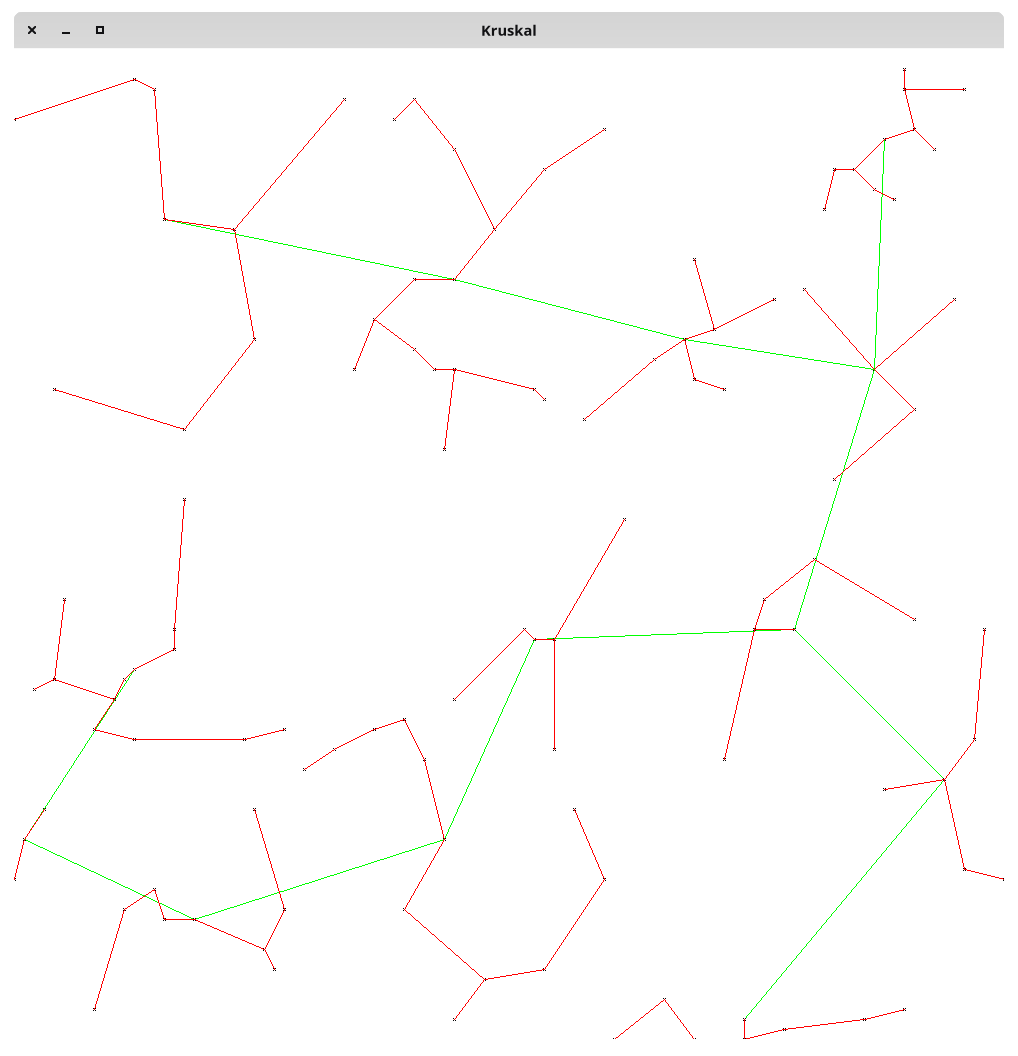
\includegraphics[width=0.5\textwidth]{k_k}
\end{frame}
\begin{frame}{Résultat de l'algorithme final}
    \centering
        \includegraphics[height=0.8\textheight]{k_k_r}
\end{frame}
\section{Conclusion}
\UseRawInputEncoding
\section{Codes}
\begin{frame}[allowframebreaks]{shortestpath.c}
    \lstinputlisting[language=C, firstline=165, lastline=197]{shortestpath.c} 
\end{frame}
\begin{frame}[allowframebreaks]{kruskal.c}
    \lstinputlisting[language=C, firstline=218, lastline=245]{kruskal.c} 
\end{frame}
\begin{frame}[allowframebreaks]{kavg.c}
    \lstinputlisting[language=C, firstline=250, lastline=286]{kavg.c} 
\end{frame}
\begin{frame}[allowframebreaks]{graph.py}
    \lstinputlisting[language=Python, firstline=46, lastline=75]{graph.py} 
\end{frame}
\end{document}